\documentclass[10pt]{article} % For LaTeX2e
\usepackage{tmlr}
% If accepted, instead use the following line for the camera-ready submission:
%\usepackage[accepted]{tmlr}
% To de-anonymize and remove mentions to TMLR (for example for posting to preprint servers), instead use the following:
%\usepackage[preprint]{tmlr}

\usepackage{hyperref}
\usepackage{url}
\usepackage{graphicx}
\usepackage{booktabs}
\usepackage{amsmath}
\usepackage{amssymb}

\title{Trust, but Verify: Cross-Conformal Auditing of Oversampling under Minority-Class Label Contamination}

% Authors must not appear in the submitted version. They should be hidden
% as long as the tmlr package is used without the [accepted] or [preprint] options.
% Non-anonymous submissions will be rejected without review.
\author{\name Muhammad Adeel Tariq \email madeelmalikdev@gmail.com \\
      \addr Department of Computer Science\\
      International Islamic University Islamabad, Islamabad, Pakistan}

\begin{document}

\maketitle

\begin{abstract}
Oversampling methods such as SMOTE create synthetic minority examples by interpolating between minority ``seed'' points. When the minority class contains mislabelled majority examples, every such fake seed spawns a synthetic neighbourhood in majority territory. Filtering remedies either delete training data, risking minority collapse, or threshold raw classifier probabilities, which we show certify most fake seeds as trustworthy. We propose CrossConfSMOTE, a SMOTE-style sampler that, to our knowledge, is the first to audit both interpolation seeds and synthetic candidates with Mondrian conformal prediction sets. Out-of-fold scores from $K$ cross-fitted scorers are pooled per class into calibration distributions, and a point is trusted only if its prediction set is exactly $\{\textit{minority}\}$. Suspicious seeds are excluded from generation only, never deleted from training, and rejected candidates are resampled. On 8 datasets, 5 noise conditions and 2 classifiers (80 blocks), CrossConfSMOTE is statistically tied with a raw-probability gate for the best average PR-AUC rank and significantly outperforms SMOTE, Borderline-SMOTE, ADASYN, SMOTEENN, class weighting, no sampling and split-conformal auditing (Holm-corrected Wilcoxon, $p \le 0.001$), as well as reimplementations of GK-SMOTE, RSMOTE and SMOTE-IPF ($p \le 1.7 \times 10^{-5}$). Its advantage over the probability gate is control rather than accuracy: against recorded ground-truth contamination, it excludes 89--92\% of fake seeds, whereas the probability gate excludes 30--37\%. The trusted seed set is 4.8\%/12.5\%/20.6\% fake at contamination levels of $0.5\times$/$1\times$/$2\times$ the minority count, versus 27.9\%/42.0\%/57.3\% for the probability gate.
\end{abstract}

\section{Introduction}

Class imbalance and label noise co-occur in many deployed minority-class problems: fraud labels arrive from disputed transactions, medical labels from fallible coders, and fault labels from incomplete logs. SMOTE \citep{chawla2002smote} and its descendants address imbalance by interpolating between minority points, implicitly assuming that the minority labels are correct. The assumption is load-bearing: a single mislabelled majority point inside the minority class acts as a seed that manufactures an entire synthetic neighbourhood in majority territory, shifting the learned boundary toward the error.

Existing remedies fall into three families. \emph{Editing and filtering} methods (ENN- and IPF-based, e.g., SMOTE-IPF \citep{saez2015smoteipf}) delete suspicious points outright; under heavy contamination they can delete much of the genuine minority, and they offer no principled knob for trading purity against retention. \emph{Geometric and density-based} methods \citep{chen2021rsmote, miraj2025gksmote} categorise seeds by local density and generate cautiously, but their categories are heuristics without error control. \emph{Confidence-based} filters (e.g., confident learning \citep{northcutt2021confident}) threshold predicted probabilities. We show empirically (Section~\ref{sec:gate}) that a single-fit probability gate certifies most injected fakes as trustworthy, because its scorer is trained on the contaminated data and has partially memorised the contamination.

Conformal prediction \citep{vovk2005algorithmic} offers what these methods lack: distribution-free, finite-sample control of an error rate at a level $\alpha$ chosen by the practitioner. Conformal prediction has been applied to learning with noisy or imbalanced data at \emph{training} time \citep{grahamknight2024conformal} and to synthesising data from high-confidence feature-space regions \citep{meister2024conformalised}, but to our knowledge it has not been used to audit the \emph{seeds and candidates of SMOTE-style interpolation} under minority-label contamination, nor evaluated against recorded ground-truth contamination. This paper addresses that gap.

\paragraph{Contributions.}
\begin{enumerate}
\item \textbf{CrossConfSMOTE}: a SMOTE-style sampler whose seed and synthetic-candidate audits are Mondrian conformal prediction sets computed from pooled out-of-fold (cross-conformal) scores, so that the minority calibration set is as large as the minority class itself; this matters under extreme imbalance, where split-conformal calibration sets are tiny.
\item A \textbf{level statement} (Section~\ref{sec:level}) for the rate at which truly-majority points are certified as minority seeds, together with an identity (Equation~\ref{eq:fdp}) that separates this controllable rate from the trusted-set contamination it induces.
\item A \textbf{benchmark protocol} with known ground-truth contamination (majority-to-minority flips at $0.5\times$/$1\times$/$2\times$ the minority count, plus minority-label loss), fold- and repeat-averaged block statistics and Holm-corrected paired tests, avoiding pseudoreplication.
\item \textbf{Gate diagnostics} against the recorded fake-seed masks: the cross-conformal gate removes about 90\% of fakes, and its trusted sets are 2.8--5.8$\times$ cleaner than those of the probability and split-conformal gates.
\end{enumerate}

\section{Related Work}

\subsection{SMOTE and noise-aware variants}

SMOTE \citep{chawla2002smote} interpolates between a minority point and one of its $k$ nearest minority neighbours. Borderline-SMOTE \citep{han2005borderline} restricts seeds to the decision border, ADASYN \citep{he2008adasyn} weights seeds by local difficulty, and SMOTEENN \citep{batista2004study} appends an editing rule. SMOTE-IPF \citep{saez2015smoteipf} iteratively filters the augmented set with an ensemble. RSMOTE \citep{chen2021rsmote} uses relative density to separate noisy, borderline and safe minority samples, and GK-SMOTE \citep{miraj2025gksmote} uses Gaussian kernel density estimates to generate in high-density regions and avoid noisy ones. Confident learning \citep{northcutt2021confident} estimates the joint distribution of noisy and true labels from cross-validated probabilities and prunes likely errors; applied before SMOTE it deletes data. Surveys of label noise are given by \citet{frenay2014classification}, and of imbalanced learning by \citet{he2009learning}.

\subsection{Conformal prediction}

Conformal prediction \citep{vovk2005algorithmic, lei2018distribution} yields set-valued predictions with finite-sample coverage. Mondrian (label-conditional) conformal prediction \citep{vovk2012conditional} calibrates per class and is the standard remedy when marginal conformal sets under-cover a rare class. Cross-conformal prediction \citep{vovk2015cross} pools out-of-fold scores to enlarge calibration sets, at the cost of a $1-2\alpha$ rather than $1-\alpha$ worst-case guarantee \citep{barber2021predictive}. Conformal p-values have also been used for outlier testing \citep{bates2023testing}.

\subsection{Conformal methods for noisy and imbalanced data}

Several works study conformal prediction \emph{under} label noise \citep{einbinder2024label, penso2024conformal}, i.e., how noisy calibration labels affect coverage. Conformal-in-the-Loop (CitL) \citep{grahamknight2024conformal} uses conformal uncertainty to re-weight and prune samples while training deep networks on imbalanced, noisy data. Conformalised data synthesis \citep{meister2024conformalised} generates data from feature-space grid points whose Mondrian conformal confidence is high. Our setting differs: we operate on tabular data at the data level, audit the specific seeds and candidates of SMOTE interpolation, never delete training points, and evaluate the audit directly against injected ground truth.

\section{Method}

\subsection{Setup}

Let $D = \{(x_i, y_i)\}$ be a binary training set with minority class $y=1$ of size $n_1$ and majority $y=0$ of size $n_0 \gg n_1$. An unknown subset of the minority-labelled points may be mislabelled majority points (``fake seeds''). The sampler must return a rebalanced set of ratio $\rho$ ($\rho = 1$ throughout) for a downstream classifier.

\subsection{Cross-conformal scores}

Split $D$ into $K=5$ stratified folds. Train scorer $f_k$ (gradient boosting) on all folds but $k$, so that every point receives an out-of-fold probability vector from a scorer that never saw it. Pool the nonconformity scores $s = 1 - \hat{p}_{y}(x)$, computed under each point's \emph{labelled} class, into per-class calibration distributions $\mathcal{C}_0, \mathcal{C}_1$. For a point $x$ (seed or candidate) and class $c$, the conformal p-value is
\begin{equation}
p_c(x) = \frac{1 + \#\{s \in \mathcal{C}_c : s \ge 1 - \hat{p}_c(x)\}}{|\mathcal{C}_c| + 1},
\end{equation}
with $\hat{p}$ taken from the out-of-fold scorer for training points and the median p-value across the $K$ fold scorers for new candidates.

\subsection{The singleton-set audit}

A point is \textbf{trusted} iff its conformal prediction set is exactly $\{1\}$, i.e., $p_1(x) > \alpha$ and $p_0(x) \le \alpha$ ($\alpha = 0.10$ throughout). The two-sided rule is essential. An early diagnostic with the one-sided rule ($p_1 > \alpha$ only) caught under 5\% of injected fakes on mammography, because calibration against the noisy minority distribution makes fakes look typical of the minority. Requiring the point to also be \emph{atypical of the majority} is what exposes them. In a preliminary split-conformal diagnostic the two-sided rule caught 43--51\% of fakes at 81--97\% gate precision. The audit is applied twice (Algorithm~\ref{alg:crossconf}):
\begin{enumerate}
\item \textbf{Seed audit.} Untrusted minority points are excluded from the generation pool. They are \emph{not} removed from the training set handed to the classifier: deletion is what collapses minorities under filtering methods, whereas exclusion from generation merely stops amplification.
\item \textbf{Synthetic audit.} SMOTE candidates are interpolated among trusted seeds only and then audited; rejected candidates are resampled until the target count is reached. A duplication fallback was triggered in fewer than 1\% of runs, and the sampler falls back to all seeds if fewer than two are trusted.
\end{enumerate}

\begin{center}
\fbox{\begin{minipage}{0.92\textwidth}
\textbf{Algorithm 1: CrossConfSMOTE}\\
\textbf{Require:} training set $D$, level $\alpha$, folds $K$, target ratio $\rho$\\
1: Fit $K$ cross-fitted scorers; obtain out-of-fold scores for all of $D$\\
2: Pool labelled-class scores into $\mathcal{C}_0, \mathcal{C}_1$\\
3: $S \leftarrow \{x \in D_{y=1} : p_1(x) > \alpha \wedge p_0(x) \le \alpha\}$ \hfill $\triangleright$ trusted seeds\\
4: \textbf{while} synthetic count $<$ target \textbf{do}\\
5: \quad Draw $x \in S$ and a minority neighbour in $S$; interpolate to $z$\\
6: \quad \textbf{if} $p_1(z) > \alpha \wedge p_0(z) \le \alpha$ \textbf{then} accept $z$\\
7: \textbf{end while}\\
8: \textbf{return} $D \cup \{\text{accepted } z\}$ \hfill $\triangleright$ no training point is deleted
\end{minipage}}
\label{alg:crossconf}
\end{center}

\subsection{Level of the audit}
\label{sec:level}

\textbf{Proposition 1.} Let $x$ be a truly-majority point whose majority nonconformity score is exchangeable with the scores of the clean majority calibration points. If $x$ is trusted then $p_0(x) \le \alpha$. Under split calibration, the standard Mondrian argument gives $\Pr(p_0(x) \le \alpha \mid y=0) \le \alpha$, hence $\Pr(x \text{ trusted} \mid y=0) \le \alpha$. Under $K$-fold cross-fitting the same event is controlled at level $2\alpha$ up to an $O(K/n)$ term, by the coverage analysis of cross-conformal prediction \citep{vovk2015cross, barber2021predictive}; the realised rate is typically close to $\alpha$.

Thus $\alpha$ governs the rate $\varphi$ at which genuine majority points (fakes) pass the audit; it does \emph{not} directly bound the fraction of fakes among trusted seeds. Let $\pi$ be the fraction of fakes in the minority-labelled pool ($\pi = m/(1+m)$ for injection level $m$), $\varphi$ the fake pass rate and $\tau$ the true-seed retention. The contamination of the trusted set (a false-discovery proportion) is
\begin{equation}
\mathrm{FDP} = \frac{\pi \varphi}{\pi \varphi + (1-\pi)\tau}.
\label{eq:fdp}
\end{equation}
At fixed $\varphi \approx \alpha$, FDP therefore rises with $\pi$ even though the audit's level is unchanged. We verify this identity empirically in Section~\ref{sec:gate}. Two caveats are part of the method: (i) the calibration pool is the \emph{labelled} data, so under contamination the effective level degrades as $\pi$ grows; and (ii) the level governs certification of majority points, not retention of minority points, which is an empirical quantity we report alongside.

\section{Experimental Protocol}

\textbf{Datasets.} Eight public binary datasets from OpenML spanning prevalence 1.4--30\% (Table~\ref{tab:datasets}); credit-g is included as a low-imbalance control. \textbf{Noise model.} Noise is injected into training folds only; test folds keep original labels and prevalence. \emph{Contamination:} $m$ majority points are relabelled minority, $m \in \{0, 0.5, 1, 2\} \times$ the training minority count (at $2\times$, two thirds of the minority-labelled pool is fake). \emph{Minority loss:} 20\% of minority labels are flipped to majority. The injected mask is recorded, enabling exact gate diagnostics. This gives five noise conditions. \textbf{Evaluation.} Stratified 5-fold cross-validation with 2 repeats; resampling is strictly inside training folds, and median imputation and standardisation are fitted on training folds only. The primary metric is PR-AUC \citep{saito2015precision}; the secondary metric is MCC at threshold 0.5. Classifiers are histogram gradient boosting (headline) and random forest. \textbf{Methods.} Thirteen sampling strategies: no sampling, class weights, SMOTE, Borderline-SMOTE, ADASYN, SMOTEENN (all via imbalanced-learn \citep{lemaitre2017imbalanced}); \emph{ProbSMOTE}, the same pipeline with a raw-probability gate in place of the conformal audit (a single scorer fit on the contaminated pool); \emph{ConfSMOTE}, a split-conformal ablation; CrossConfSMOTE; its seed-only ablation; and our reimplementations of GK-SMOTE, RSMOTE and SMOTE-IPF (original code unavailable).

\textbf{Statistics.} Scores are averaged over folds and repeats to one value per (dataset $\times$ condition $\times$ classifier) block ($N=80$) before any test; folds are never treated as independent samples. We use a Friedman omnibus test and pairwise Wilcoxon signed-rank tests with Holm correction \citep{demsar2006statistical, holm1979simple}, with effect sizes as mean paired PR-AUC differences and win counts reported.

\begin{table}[t]
\caption{Datasets (instances $\times$ features, minority prevalence).}
\label{tab:datasets}
\begin{center}
\begin{tabular}{lcc}
\toprule
Dataset & $n \times d$ & Minority \\
\midrule
mammography & 11,183 $\times$ 6 & 2.3\% \\
satellite & 5,100 $\times$ 36 & 1.5\% \\
sick & 3,772 $\times$ 53 & 6.1\% \\
ozone-level-8hr & 2,534 $\times$ 72 & 6.3\% \\
yeast\_ml8 & 2,417 $\times$ 116 & 1.4\% \\
pc1 & 1,109 $\times$ 21 & 6.9\% \\
credit-g (one-hot) & 1,000 $\times$ 61 & 30.0\% \\
oil spill & 937 $\times$ 49 & 4.4\% \\
\bottomrule
\end{tabular}
\end{center}
\end{table}

\section{Results}

\subsection{Downstream performance}

Table~\ref{tab:ranks} gives average ranks among the ten primary methods, and Figure~\ref{fig:ranks} shows all thirteen. CrossConfSMOTE ranks first among the ten primary methods (3.79) but is statistically indistinguishable from ProbSMOTE (3.81; Holm $p = 0.375$). Across all thirteen methods the order flips (ProbSMOTE 4.47, CrossConfSMOTE 4.53). We therefore make no claim of accuracy superiority over the probability gate. Against every other rival the advantage is significant after Holm correction (Table~\ref{tab:ranks}): SMOTE $+0.019$ PR-AUC, Borderline-SMOTE $+0.024$, ADASYN $+0.032$, SMOTEENN $+0.049$, class weights $+0.023$, no sampling $+0.015$, split-conformal ConfSMOTE $+0.011$. The seed-only ablation is significantly worse than the full method ($+0.0016$, $p_{\mathrm{Holm}} = 0.026$), so both audits contribute. Against the prior-art reimplementations (Table~\ref{tab:priorart}) CrossConfSMOTE wins clearly. On MCC at the fixed 0.5 threshold it also beats no sampling ($+0.024$, 46/80 blocks), so the ranking advantage is not an artefact of threshold choice. Per-condition ranks are best or near-best where the method is designed to matter: contamination $0.5\times$ (3.38), $1\times$ (2.94) and $2\times$ (3.50). It is mid-pack on clean data (4.62) and minority loss (4.50), where the probability gate is comparable. ADASYN failed to produce samples on credit-g at $0.5\times$ contamination in all folds (an imbalanced-learn sampling-ratio error); we report this cell as failed rather than imputing it.

\begin{table}[t]
\caption{Average PR-AUC ranks among the ten primary methods over 80 blocks (lower is better) and Holm-corrected Wilcoxon tests of CrossConfSMOTE versus each rival. $\Delta$ is the mean PR-AUC advantage of CrossConfSMOTE.}
\label{tab:ranks}
\begin{center}
\begin{tabular}{lccc}
\toprule
Method & Avg.\ rank & $\Delta$ PR-AUC & $p_{\mathrm{Holm}}$ \\
\midrule
CrossConfSMOTE & 3.79 & --- & --- \\
ProbSMOTE (control) & 3.81 & $+0.002$ & 0.375 (n.s.) \\
CrossConf (seed-only) & 4.41 & $+0.002$ & 0.026 \\
ConfSMOTE (split) & 5.18 & $+0.011$ & 0.0001 \\
No sampling & 5.21 & $+0.015$ & 0.001 \\
SMOTE & 5.80 & $+0.019$ & 0.0002 \\
Class weights & 6.02 & $+0.023$ & $<0.0001$ \\
Borderline-SMOTE & 6.35 & $+0.024$ & $<0.0001$ \\
ADASYN & 7.05 & $+0.032$ & $<0.0001$ \\
SMOTEENN & 7.30 & $+0.049$ & $<0.0001$ \\
\bottomrule
\end{tabular}
\end{center}
\end{table}

\begin{table}[t]
\caption{CrossConfSMOTE versus reimplementations of prior art (80 blocks).}
\label{tab:priorart}
\begin{center}
\begin{tabular}{lccc}
\toprule
Method & $\Delta$ PR-AUC & Blocks won & $p$ \\
\midrule
GK-SMOTE* & $+0.019$ & 58/80 & $1.6 \times 10^{-5}$ \\
RSMOTE* & $+0.015$ & 61/80 & $1.3 \times 10^{-5}$ \\
SMOTE-IPF* & $+0.047$ & 62/80 & $5.6 \times 10^{-9}$ \\
\bottomrule
\end{tabular}
\end{center}
{\small * Our reimplementation of the published algorithm.}
\end{table}

\begin{figure}[t]
\begin{center}
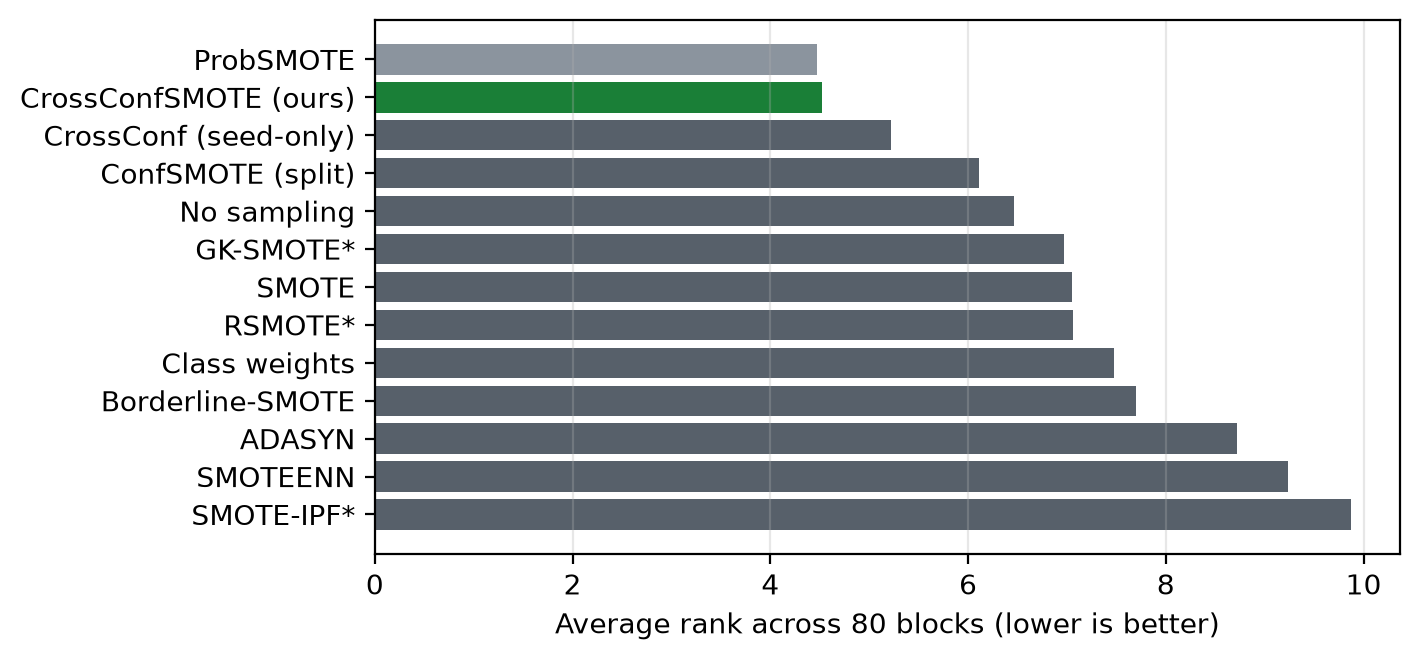
\includegraphics[width=0.92\textwidth]{fig_ranks.png}
\end{center}
\caption{Average ranks over 80 blocks, all 13 methods. * = our reimplementation of the published algorithm.}
\label{fig:ranks}
\end{figure}

\subsection{Gate quality: the decisive diagnostic}
\label{sec:gate}

Downstream metrics cannot distinguish \emph{why} a gate helps. Because the noise injection is recorded, we can score the gates directly (4 datasets $\times$ 5 folds $\times$ 3 contamination levels; Table~\ref{tab:gate}, Figure~\ref{fig:gate}). The cross-conformal gate excludes 89--92\% of injected fakes while retaining 78--84\% of true seeds for generation. The probability gate excludes only 30--37\% of fakes and the split-conformal gate 28--29\%. Consequently the trusted seed set, the raw material of every synthetic point, is 4.8\% fake at $0.5\times$ contamination for CrossConfSMOTE versus 27.9\% (probability) and 27.1\% (split-conformal), and at $2\times$ it is 20.6\% versus 57.3\% and 59.9\%. The laxer gates retain more true seeds (89--96\%), but what they retain is poisoned: seed purity, not seed count, is the binding constraint, which is why the stricter gate wins or ties downstream despite discarding about a fifth of the true seeds from generation.

\emph{Relation to the nominal level.} The fake pass rate of the cross-conformal gate, $\varphi = 1 - \mathrm{recall}$, is 8.4\%, 11.2\% and 9.9\% at the three levels, close to $\alpha = 0.10$, whereas the probability and split-conformal gates pass 63--72\% of fakes. The rising trusted-set contamination is therefore not a failure of the level: it is the base-rate effect of Equation~\ref{eq:fdp}. Table~\ref{tab:fdp} shows that Equation~\ref{eq:fdp}, evaluated on the mean $\varphi$ and $\tau$ of Table~\ref{tab:gate}, reproduces the observed contamination to within 0.013 for all nine gate--level combinations. Why do the single-fit gates fail? Their scorer is trained on the contaminated pool and partially memorises it, so a fake seed's own neighbourhood votes for it. Cross-fitting breaks this self-endorsement: every point is judged by a model that never trained on it, and conformal calibration converts that judgement into a level-$\alpha$ decision rather than a threshold on an uncalibrated probability. Because our probability and split-conformal gates differ from CrossConfSMOTE in more than one respect, this diagnostic does not by itself isolate which ingredient (cross-fitting, class-conditional calibration, or the two-sided rule) is responsible; see Section~\ref{sec:discussion}.

\begin{table}[t]
\caption{Gate diagnostics against known injected fake seeds (means over 4 datasets $\times$ 5 folds). Trusted-set contamination is the fraction of generation-trusted seeds that are actually fake.}
\label{tab:gate}
\begin{center}
\begin{tabular}{llccc}
\toprule
Level & Gate & Fake recall & True-seed ret. & Contam. \\
\midrule
$0.5\times$ & CrossConf & 0.916 & 0.840 & 0.048 \\
 & Probability & 0.304 & 0.890 & 0.279 \\
 & Split-conf. & 0.279 & 0.961 & 0.271 \\
$1\times$ & CrossConf & 0.888 & 0.807 & 0.125 \\
 & Probability & 0.339 & 0.895 & 0.420 \\
 & Split-conf. & 0.286 & 0.954 & 0.426 \\
$2\times$ & CrossConf & 0.901 & 0.781 & 0.206 \\
 & Probability & 0.371 & 0.890 & 0.573 \\
 & Split-conf. & 0.289 & 0.939 & 0.599 \\
\bottomrule
\end{tabular}
\end{center}
\end{table}

\begin{table}[t]
\caption{Check of Equation~\ref{eq:fdp}: predicted versus observed trusted-set contamination ($\pi = m/(1+m)$).}
\label{tab:fdp}
\begin{center}
\begin{tabular}{llccc}
\toprule
Level ($\pi$) & Gate & $\varphi$ & Predicted & Observed \\
\midrule
$0.5\times$ (0.333) & CrossConf & 0.084 & 0.048 & 0.048 \\
 & Probability & 0.696 & 0.281 & 0.279 \\
 & Split-conf. & 0.721 & 0.273 & 0.271 \\
$1\times$ (0.500) & CrossConf & 0.112 & 0.122 & 0.125 \\
 & Probability & 0.661 & 0.425 & 0.420 \\
 & Split-conf. & 0.714 & 0.428 & 0.426 \\
$2\times$ (0.667) & CrossConf & 0.099 & 0.202 & 0.206 \\
 & Probability & 0.629 & 0.586 & 0.573 \\
 & Split-conf. & 0.711 & 0.602 & 0.599 \\
\bottomrule
\end{tabular}
\end{center}
\end{table}

\begin{figure}[t]
\begin{center}
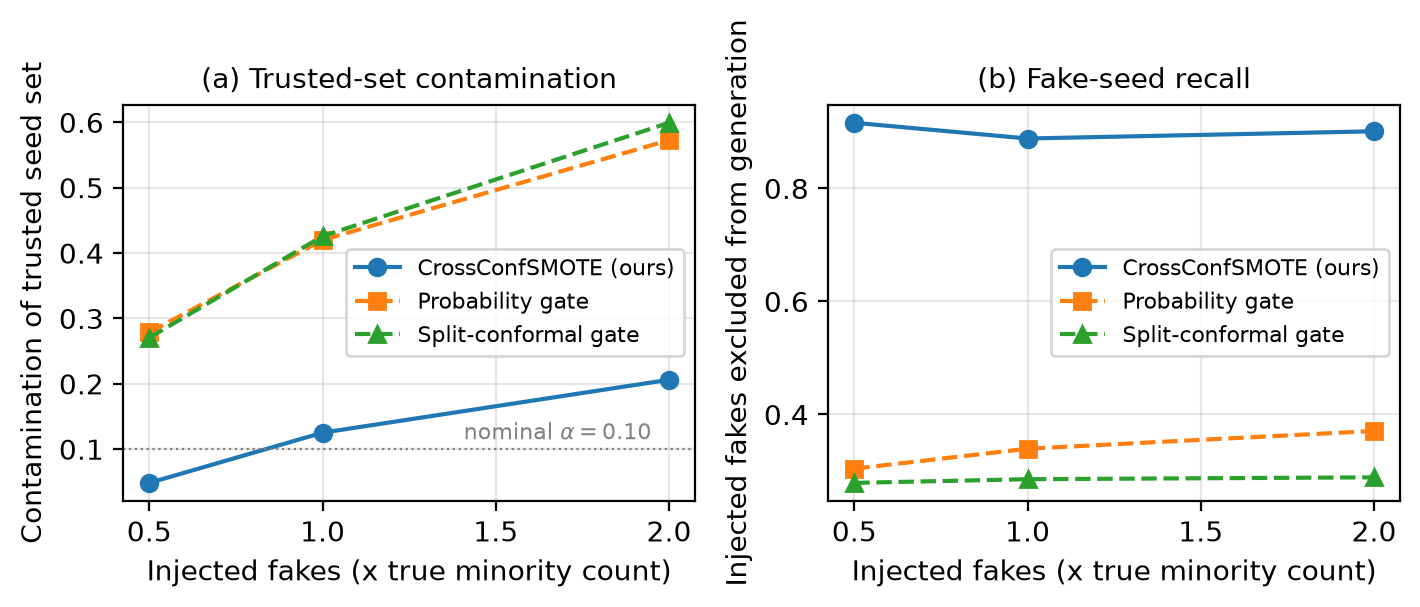
\includegraphics[width=0.95\textwidth]{fig_gate.png}
\end{center}
\caption{Gate diagnostics versus injected contamination. (a) Fraction of the trusted seed set that is fake; the dotted line is the nominal level $\alpha = 0.10$, which controls the fake pass rate but not, directly, this fraction. (b) Fraction of injected fake seeds excluded from generation.}
\label{fig:gate}
\end{figure}

\section{Discussion and Limitations}
\label{sec:discussion}

CrossConfSMOTE's contribution is control, not a new accuracy frontier: a practitioner chooses $\alpha$ and obtains a gate whose fake pass rate is near that level, with trusted-set contamination predictable from Equation~\ref{eq:fdp}, instead of hoping that a 0.5 probability threshold means something. The limitations are as follows.

\begin{enumerate}
\item The level statement assumes clean-calibration exchangeability; real contamination violates it in proportion to its level, which our diagnostics quantify but do not eliminate. The cross-fitted variant is covered by a $2\alpha$ guarantee inherited from cross-conformal analyses, not a bespoke proof for the exact pooling used here.
\item The gate discards 16--22\% of true seeds from generation; at extremely small minority counts this could starve generation (the sampler then falls back to all seeds).
\item The downstream advantage over the probability gate is a tie on these benchmarks. Moreover, our probability gate is single-fit, so the comparison does not separate the contribution of cross-fitting from that of conformal calibration; a cross-fitted probability-threshold gate, which resembles confident learning, is the natural further control. Domains where the scorer is weaker or contamination is structured differently may separate the methods in either direction.
\item Contamination is injected by uniformly relabelling majority points, which is class-conditional and feature-independent; instance-dependent noise that places fakes near the boundary is harder and is not studied here.
\item The gate diagnostics cover 4 of the 8 datasets, and the minority-loss condition has no gate diagnostic.
\item GK-SMOTE, RSMOTE and SMOTE-IPF numbers come from our reimplementations of the published algorithms.
\item Runtime is roughly $K\times$ the scorer cost of SMOTE: negligible at these scales, but relevant at web scale.
\end{enumerate}

\section{Conclusion}

Oversampling amplifies whatever it is fed, including label errors. Auditing the feed with cross-conformal prediction sets, excluding suspicious seeds from generation without deleting them and resampling rejected synthetics, keeps the fake pass rate near a practitioner-chosen level and matches or beats the strongest existing samplers across 80 benchmark blocks, while producing far cleaner trusted seed sets than probability and split-conformal gates. Code, data splits, injected masks and per-fold results accompany this paper as supplementary material so that every reported number can be checked.

\subsubsection*{Reproducibility Statement}

All datasets are public (OpenML). The sampler, experiment runners, injected contamination masks, per-fold results and the analysis scripts that produce every table and figure in this paper are submitted as anonymised supplementary material. All experiments use fixed seeds, resampling strictly inside training folds, and fold- and repeat-averaged block statistics, so every reported number can be recomputed from the released artefacts.

\bibliography{crossconfsmote}
\bibliographystyle{tmlr}

\end{document}
